
\documentclass{article}
\usepackage{url}
\usepackage{graphicx,subfigure}
\usepackage{xspace}

\newcommand{\ie}{{\em i.e.,}~}
\newcommand{\eg}{{\em e.g.,}~}


\title{Consumer Review Analysis with Linear Regression}

%\numberofauthors{1}
\author{Cliff Engle \and Antonio Lupher}

\begin{document}


%%%%%%%%%%%%%%%%%%%%%%%%%%%%%%%%%%%%%%%%%%%%%%%%%%%%%%%%%%%%%%%%%%%%%%%%%%%%%%%
%%%%%%%%%%%%%%%%%%%%%%%%%%%%%%%%%%%%%%%%%%%%%%%%%%%%%%%%%%%%%%%%%%%%%%%%%%%%%%%
%%%%%%%%%%%%%%%%%%%%%%%%%%%%%%%%%%%%%%%%%%%%%%%%%%%%%%%%%%%%%%%%%%%%%%%%%%%%%%%

\maketitle

\section{Introduction}
Sentiment analysis aims to classify people's sentiments towards a particular subject based on their opinions. There are a number of different classification methods that can be used to perform this analysis. In this paper, we perform sentiment analysis on a labeled dataset of Amazon product reviews using linear regression. The dataset consists of one million textual reviews, of which approximately 500,000 are unique. We perform 10-fold cross-validation of our linear regression method, and experiment with various configuration parameters to provide optimal performance.

\section{Linear Regression}
Linear regression is a method to model the relationship between an output variable, $y$, and explanatory variables, $X$. The output variable is a linear sum of the explanatory variables multiplied by their corresponding coeffecients, represented by $\beta$. In our case, $y$ represents a review's ranking from one to five, while $X$ is the bag-of-words representation of the review text. This implies that $\beta$ represents the weight of a word's correlation to a higher review. This gives us the simple regression formula: $$y=X\beta$$

In this paper, we perform ordinary least squares regression. By minimizing the sum of squared residuals, we can solve for the unkown parameter vector $\beta$ using a closed form solution. $$\beta=(X'X)^{-1}X'y$$ In order to ensure that the matrix $X'X$ is invertible, we perform ridge regression. In ridge regression, we add the identity matrix, $I$, scaled by a factor, $\lambda$, to produce the following equation. $$\beta=(X'X+\lambda I)^{-1}X'y$$ We calculate this $\beta$ for a training set of review text along with their corresponding ratings which range from 1 to 5. We then evaluate our model $\beta$ on the withheld reviews in order to perform a 10 fold cross validation.

%%%%%%%%%%%%%%%%%%%%%%%%%%%%%%%%%%%%%%%%%%%%%%%%%%%%%%%%%%%%%%%%%%%%%%%%%%%%%%%
%%%%%%%%%%%%%%%%%%%%%%%%%%%%%%%%%%%%%%%%%%%%%%%%%%%%%%%%%%%%%%%%%%%%%%%%%%%%%%%
%%%%%%%%%%%%%%%%%%%%%%%%%%%%%%%%%%%%%%%%%%%%%%%%%%%%%%%%%%%%%%%%%%%%%%%%%%%%%%%

\section{Implementation}
All of our code was implemented in MATLAB because of its ease-of-use and optimizations on matrix multiplications. We parsed the reviews from the tokenized binary format into a bag-of-words representation stored as a sparse matrix. Matlab uses Compressed Sparse Column format, so we actually stored the matrix $X'$ because the dictionary is very sparse. We also filtered out duplicate reviews by hashing the first ten words in a review to determine distinctness. This filtered the one million reviews to 492,130.

% Talk about stemming and stop-words

The actual matrix multiplications were done using the sparse $X$ matrix along with our $y$ vector and the ridge parameter. The multiplication $X'X$ takes up too much memory if we use the entire dictionary, so we chose to limit the dictionary size. We found that a dictionary of the 10,000 most frequent words gave sufficient features while also being computable using MATLAB's built-in sparse matrix multiplications.

\section{Design Decisions}

\begin{figure}[t]
	\centering
	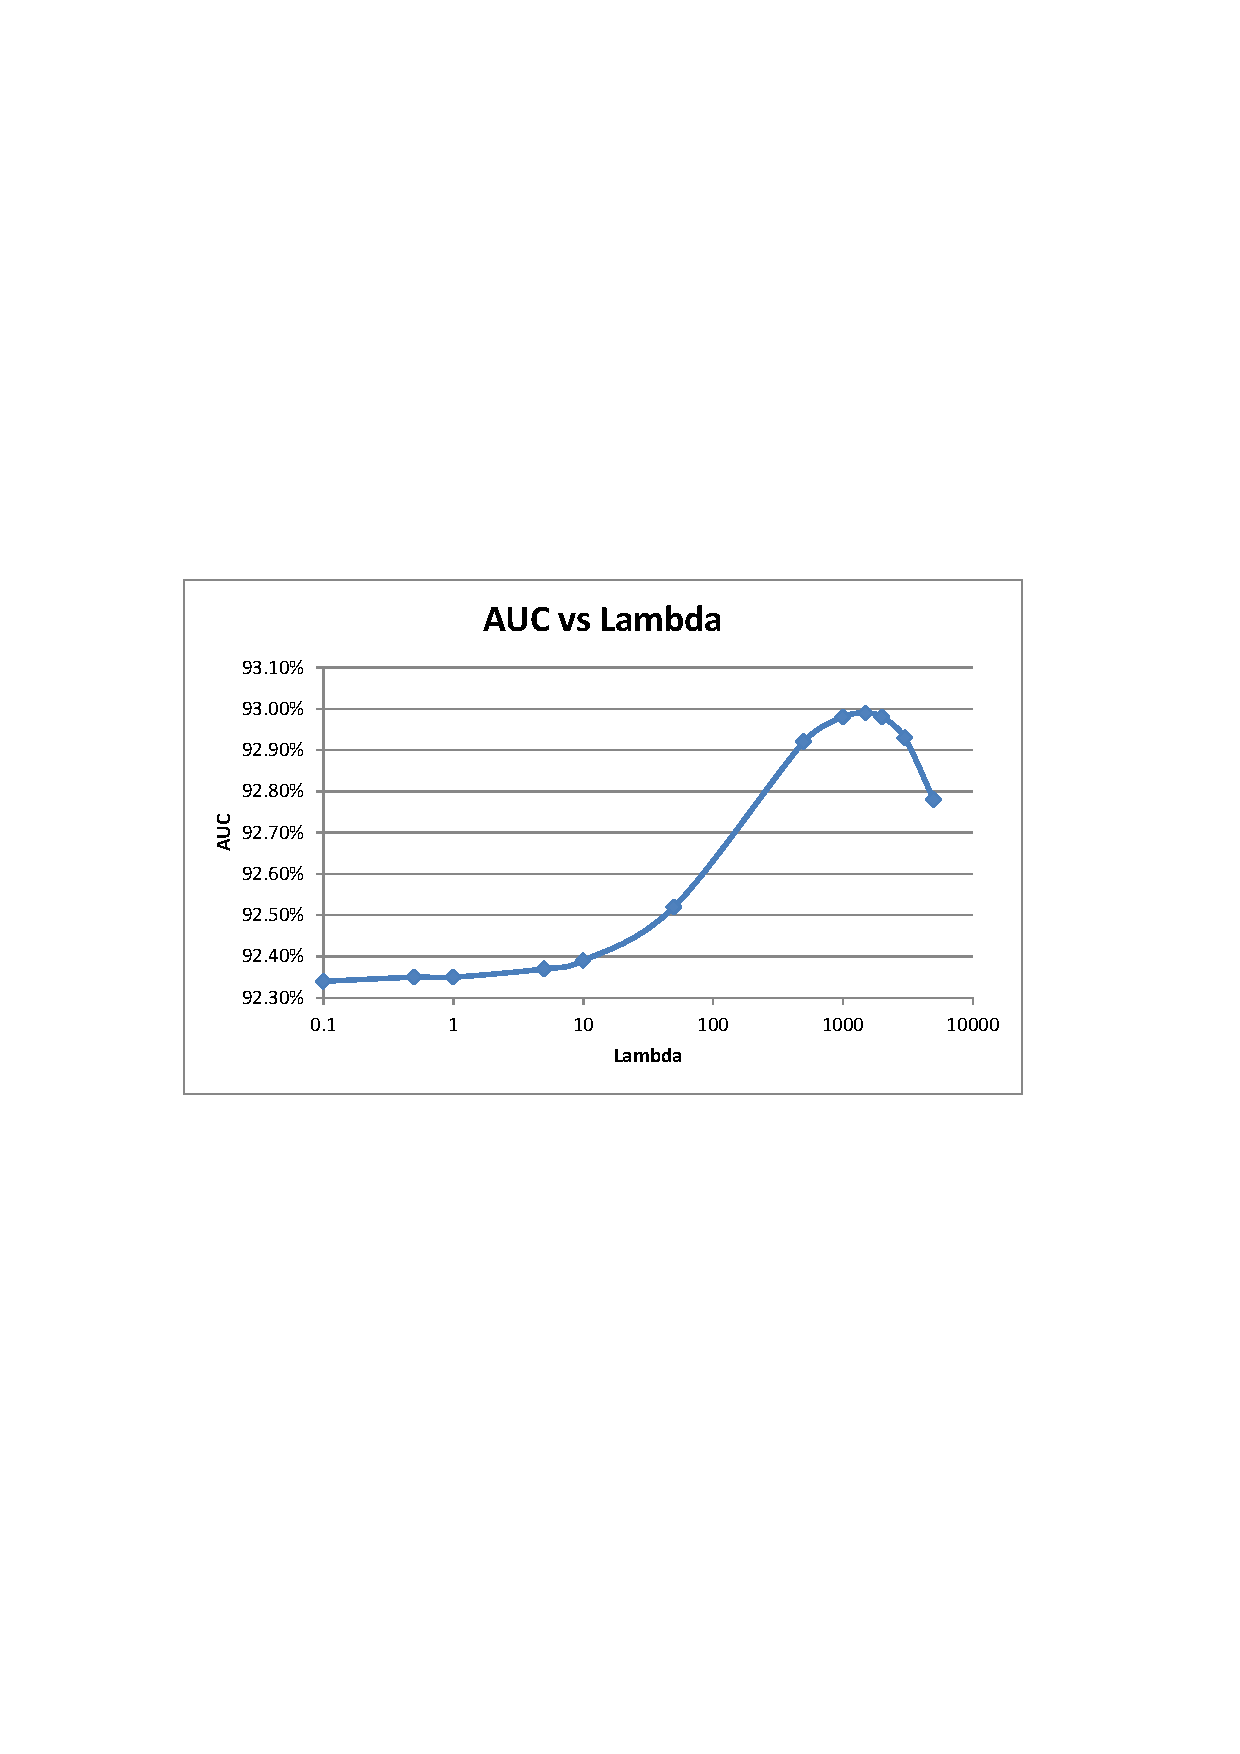
\includegraphics[width=\linewidth]{files/lambda.pdf}
	\caption{AUC based on varying lambda values for Ridge Regression. Dictionary is pruned to 15,000 words.}
	\label{fig:lambda}
\end{figure}



\subsection{Tuning the Lambda parameter}

\subsection{Porter Stemming}
Porter Stemming is a process for removing some of the common morphological and inflexional endings from words. The ramifications of this in a classifier is that it consolidates words with similar semantics. This can often help to reduce dependencies between similar words. We ran performance tests with and without Porter Stemming. 

\subsection{Stop Words}



\section{Results}

\section{Analysis}
\subsection{Top Words}

\begin{table}
    \begin{tabular}{|l|l|l|l|}
        \hline
        Top Positive Words & Weights & Top Negative Words & Weights \\ \hline
        excellent   & 0.20 & waste          & -0.71 \\ 
        awesome     & 0.18 & disappointing  & -0.57 \\ 
        invaluable  & 0.15 & poorly         & -0.56 \\ 
        highly      & 0.15 & disappointment & -0.52 \\ 
        amazing     & 0.15 & worst          & -0.47 \\ 
        outstanding & 0.15 & boring         & -0.46 \\ 
        wonderful   & 0.14 & disappointed   & -0.46 \\ 
        loved       & 0.14 & useless        & -0.42 \\ 
        pleased     & 0.14 & hoping         & -0.32 \\ 
        fantastic   & 0.14 & lacks          & -0.31 \\
        \hline
    \end{tabular}
    \caption{Top words and their weights using a lambda of 1500}
    \label{tab:words}
\end{table}


%%%%%%%%%%%%%%%%%%%%%%%%%%%%%%%%%%%%%%%%%%%%%%%%%%%%%%%%%%%%%%%%%%%%%%%%%%%%%%%
%%%%%%%%%%%%%%%%%%%%%%%%%%%%%%%%%%%%%%%%%%%%%%%%%%%%%%%%%%%%%%%%%%%%%%%%%%%%%%%
%%%%%%%%%%%%%%%%%%%%%%%%%%%%%%%%%%%%%%%%%%%%%%%%%%%%%%%%%%%%%%%%%%%%%%%%%%%%%%%
\section{Future Improvements}




%%%%%%%%%%%%%%%%%%%%%%%%%%%%%%%%%%%%%%%%%%%%%%%%%%%%%%%%%%%%%%%%%%%%%%%%%%%%%%%
%%%%%%%%%%%%%%%%%%%%%%%%%%%%%%%%%%%%%%%%%%%%%%%%%%%%%%%%%%%%%%%%%%%%%%%%%%%%%%%
%%%%%%%%%%%%%%%%%%%%%%%%%%%%%%%%%%%%%%%%%%%%%%%%%%%%%%%%%%%%%%%%%%%%%%%%%%%%%%%

%%%%%%%%%%%%%%%%%%%%%%%%%%%%%%%%%%%%%%%%%%%%%%%%%%%%%%%%%%%%%%%%%%%%%%%%%%%%%%%
%%%%%%%%%%%%%%%%%%%%%%%%%%%%%%%%%%%%%%%%%%%%%%%%%%%%%%%%%%%%%%%%%%%%%%%%%%%%%%%
%%%%%%%%%%%%%%%%%%%%%%%%%%%%%%%%%%%%%%%%%%%%%%%%%%%%%%%%%%%%%%%%%%%%%%%%%%%%%%%




\end{document}
